\section{Virtual Private Cloud}

\begin{frame}
	\frametitle{Virtual Private Cloud (VPC)}
	\begin{itemize}
		\item VPCs são usadas para criar redes virtuais
		\item VPCs podem usar CIDR entre /16 até /28
		\item Cada região tem uma VPC padrão
			\begin{itemize}
				\item Não é recomendado usar
			\end{itemize}
		\item VPCs são isoladas entre si
			\begin{itemize}
				\item Podem ser configuradas para se comunicarem
			\end{itemize}
		\item \textbf{VPC wizard} tem algumas configurações pré-definidas de VPC
		\item Lembrar de verificar e configurar:
		\begin{itemize}
			\item DHCP options set
			\item DNS resolution
			\item DNS hostname
		\end{itemize}
	\end{itemize}
\end{frame}

\begin{frame}
	\frametitle{Conexões VPN}
	\begin{itemize}
		\item \textbf{AWS Hardware VPN}: Conexão da VPC para uma rede remota usando IPsec hardware VPN
		\item \textbf{AWS Direct Connect}: Conexão privada dedicada da VPC para uma rede remota
		\item \textbf{AWS VPN CloudHub}: Múltiplos \textbf{AWS Hardware VPN} pelo VPC permitindo comunicação entre muitas redes remotas
		\item \textbf{Software VPN}: Conexão VPN usando uma instância EC2 rodando um software VPN
	\end{itemize}
\end{frame}

\begin{frame}[allowframebreaks]
	\frametitle{Subnets}
	\begin{itemize}
		\item Subnets são uma parte da rede inteira
			\begin{itemize}
				\item A rede pode ser dividida em subnets
				\item Uma subnet pode ser dividida em subnets
			\end{itemize}
		\item Cada subnet é como uma rede separada
	\end{itemize}
	\hfill
	\begin{figure}[htpb]
	\begin{center}
	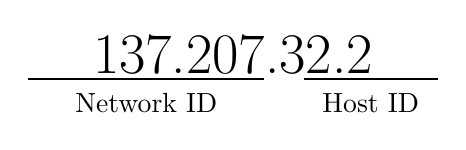
\begin{tikzpicture}[scale=1, transform shape]
		\node at (0,0) {\huge 137.207.32.2};
		\node at (1.75,-0.6) {Host ID};
		\draw (2.6,-0.3)--(0.9,-0.3);
		\node at (-1.1,-0.6) {Network ID};
		\draw (0.4,-0.3)--(-2.6,-0.3);
	\end{tikzpicture}
	\end{center}
	\caption{Subnet Addresses}
	\end{figure}
	\framebreak
	\begin{itemize}
		\item Subnets são aplicadas em AZs
		\item Subnet:
			\begin{itemize}
				\item Pública: recursos que não devem ser acessíveis pela internet
				\item Privada: recursos que devem ser acessíveis pela internet
			\end{itemize}
	\end{itemize}
\end{frame}

\begin{frame}[allowframebreaks]
	\frametitle{NAT Gateway}
	\begin{itemize}
		\item Instâncias dentro de subnets privadas podem conectar com serviços fora da VPC, mas instâncias de fora não podem iniciar ocnexões com essas instâncias
			\begin{itemize}
				\item Public: Instâncias em subnets privadas podem conectar com a internet
				\item Private: Instâncias em subnets privadas podem conectar com outros VPCs
			\end{itemize}
		\item Cobrança por hora de uso e quantidade em GBs de dados processados
	\end{itemize}
	\framebreak
	\begin{table}[htpb]
		\centering
		\caption{VPC NAT Gateway Vs NAT Instances on amazon EC2}
		\begin{tabular}{|c|c|c|}
			\hline
			& VPC NAT Gateway & NAT Instance \\
			\hline \hline
			Availability & Highly available by default & Use script to manage failover \\
			\hline
			Bandwidth & Bursts to 10 Gbps & Based on bandwidth of instance type \\
			\hline
			Maintenance & Managed by AWS & Managed by you \\
			\hline
			Security & NACLs & Security groups and NACLs \\
			\hline
			Port forwarding & Not supported & Supported \\
			\hline
		\end{tabular}
	\end{table}
\end{frame}
\begin{frame}
	\frametitle{Internet Gateway}
	\begin{itemize}
		\item Permite a comunicação do seu VPC com a internet
		\item São escaláveis horizontalmente, redundantes e tem alta disponibilidade por padrão
		\item Libera a entrada e a saída de determinado \textbf{Route Table}
		\item Não tem custo
	\end{itemize}
\end{frame}

\begin{frame}
	\frametitle{Route table}
	\begin{itemize}
		\item Determina para onde o tráfico de rede é roteado
		\item Associa as \textbf{subnets}
		\item Se a \textbf{Route table} não tiver uma rota default ela não está pública
		\item Apenas uma route table por subnet
		\item Boa prática:
			\begin{itemize}
				\item User route tables customizadas para cada subnet roteamento mais granularizado para os destinos
			\end{itemize}
	\end{itemize}
\end{frame}

\begin{frame}[allowframebreaks]
	\frametitle{Security Groups}
	\begin{itemize}
		\item Firewall virtual para controlar entrada e saída de tráfico (1 ou mais instâncias)
		\item Pode ser aplicado a um CIDR ou outro security group para situações de autoscaling
		\item Apenas regras de liberação
		\item Stateful: se o tráfego de entrada é permitido, a resposta de saída não precisa ser inspecionada/localizada e vice versa
		\item Por padrão todas os tráfegos de saída são permitidos
			\begin{itemize}
				\item Modificar a saída traz complexidade para a aplicação e não é recomendada (Apenas se for preciso por compliance)
			\end{itemize}
		\framebreak
		\item Grande parte das empresas criam security groups para cada camada da aplicação

	\end{itemize}
	\begin{figure}[htpb]
		\centering
			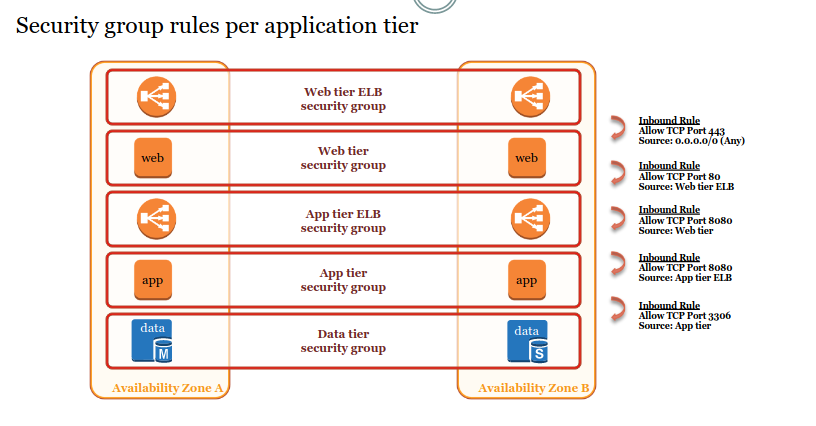
\includegraphics[width=0.8\textwidth]{vpc-security-groups-chaining}
		\caption{Security Group chaining diagram}
	\end{figure}
\end{frame}

\begin{frame}[allowframebreaks]
	\frametitle{NetworkACL}
	\begin{itemize}
		\item Regra de segurança da rede (Como se fosse um \textit{firewall})
		\item Regras de liberação e negação
		\item Stateless: o tráfego de retorno deve ser explicitamente permitido pelas regras
		\item Aplica a todas as instâncias nas sub-redes
		\item São Firewalls virtuais opcionais que controlam a entrada e a saída e uma subnet
		\item stateless: Allow all incoming/outgoing traffic by default and use stateless rules to allow or deny traffic. "Stateless rules” inspect all inbound and outbound traffic and do not keep track of connections.
		\item Cada regra vai ter uma prioridade
		\item É bom deixar um espaço entre cada regra para possíveis regras futuras (Ex: deixar 10 espaços entre cada regra)
		\item \textbf{OBS}: É bom liberar portas efêmeras (1024-65535). São usadas para comunicações de saída através do protocolo de rede TCP/IP
	\end{itemize}
\end{frame}

\begin{frame}
	\frametitle{Amazon VPC Flow Logs}
	\begin{itemize}
		\item Captura detalhes do tráfico na VPC (Aceito e recusado)
		\item Pode ser habilitado para PVCs, subnets e ENIs
		\item Uso em:
			\begin{itemize}
				\item Troubleshoot de conexões
				\item Testar regras de acesso de rede
				\item Monitorar tráfego
				\item Detectar e investigar incidentes de segurança
			\end{itemize}
	\end{itemize}
\end{frame}

\begin{frame}[allowframebreaks]
	\frametitle{AWS Infrastructure Patterns}
	\begin{figure}[htpb]
		\centering
		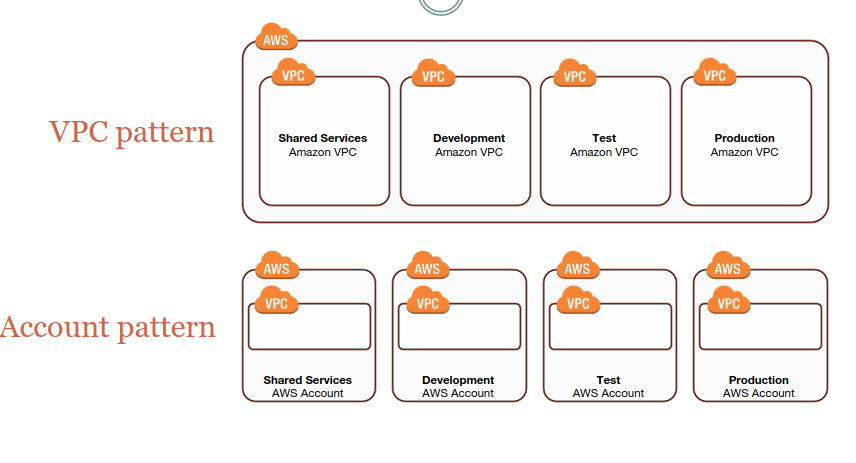
\includegraphics[width=0.8\textwidth]{aws-infra-patterns}
		\caption{VPC pattern and Account pattern\cite{FrisbyMcgibney}}
	\end{figure}
	\framebreak
	\begin{itemize}
		\item Como escolher um padrão?
			\begin{itemize}
				\item Complexidade da empresa e isolamento dos workloads
				\item Uma equipe de TI?
					\begin{itemize}
						\item Multi-VPC
					\end{itemize}
				\item Muitas equipes de TI?
					\begin{itemize}
						\item Multi-account
					\end{itemize}
				\item Alto isolamento de workload
					\begin{itemize}
						\item Multi-account
					\end{itemize}
			\end{itemize}
	\end{itemize}
\end{frame}

\begin{frame}[allowframebreaks]
	\frametitle{Network Optimization}
	\begin{itemize}
		\item Tamanho da VPC
			\begin{itemize}
				\item Evitar alocar /16 endereços IP padrão para todas as subnets
				\item Alguns recursos precisam de IPs livres 
					\begin{itemize}
						\item Ex: Load balancer precisa de 8 IPs livres)
					\end{itemize}
				\item IPAM (VPC IP Address Manager)\footnote{\href{https://aws.amazon.com/blogs/aws/network-address-management-and-auditing-at-scale-with-amazon-vpc-ip-address-manager/}{Network Address Management and Auditing at Scale with Amazon VPC IP Address Manager}} para gerenciar os IPs nas redes
					\begin{itemize}
						\item OBS: IPAM pode ser usado no CloudWatch (Verificar se os endereços IPs estão acabando ou overlay de VPC)
					\end{itemize}
			\end{itemize}
		\framebreak
		\item Quantas subnets por VPC?
			\begin{itemize}
				\item Pelo menos 1 subnet por VPC
				\item Aplicação em várias AZs = pelo menos uma subnet por AZ
					\begin{itemize}
						\item OBS: Quando uma subnet é colocada em uma AZ não é possível mudar
					\end{itemize}
			\end{itemize}
		\item Compartilhar VPC ou criar uma VPC nova para o workload?
			\begin{itemize}
				\item Times em diferentes contas da AWS, não precisam necessariamente usar diferentes VPCs
					\begin{itemize}
						\item VPC Sharing\footnote{\href{https://aws.amazon.com/blogs/networking-and-content-delivery/vpc-sharing-a-new-approach-to-multiple-accounts-and-vpc-management/}{VPC Sharing}} permite compartilhar VPCs com outras contas AWS
					\end{itemize}
				\item \href{https://aws.amazon.com/blogs/networking-and-content-delivery/vpc-sharing-key-considerations-and-best-practices/}{VPC Sharing Best Pratices}
			\end{itemize}
	\end{itemize}
\end{frame}

\begin{frame}
	\frametitle{Extra}
	\begin{itemize}
		\item Grande parte dos serviços da AWS não usam VPC
			\begin{itemize}
				\item Para esses serviços a VPC não consegue trazer nenum isolamento fora AAAAAAAAAAAAAAAA
				\item O tráfico de rede entre regiões da AWS atravessam a rede global da AWS por padrão
				\item Amazon S3 e DynamoDB oferecem VPC endpoints para conectar  sem atravessar a internet pública
			\end{itemize}
	\end{itemize}
\end{frame}

\begin{frame}
	\frametitle{Directing Traffic To Your VPC}
	\begin{itemize}
		\item To enable access to or from the Internet for instances in a VPC subnet, you must:
		\item Attach an Internet gateway to your VPC
		\item Ensure that your subnet's route table points to the Internet gateway
		\item Ensure that instances in your subnet have public IP addresses or
Elastic IP addresses
		\item  Ensure that your NACLs and security groups allow the relevant
traffic to flow to and from your instance
	\end{itemize}
\end{frame}
